\documentclass[notes=hide,hyperref={dvipdfmx,pdfpagelabels=false}]{beamer}
\mode<article>
{
  \usepackage{fullpage}
  \usepackage{pgf}
  \usepackage{hyperref}
  \setjobnamebeamerversion{beamer}
}

\mode<presentation>
{
  %\usetheme{Frankfurt}
 %\usetheme{My}
  \usetheme{Madrid}
  % or ...
%\usecolortheme{seagull}
  %\setbeamercovered{transparent}
  %\setbeamercovered{dynamic}
  % or whatever (possibly just delete it)
}
\usenavigationsymbolstemplate{}
\usefonttheme{structurebold}
\usepackage{multimedia}
\usepackage{tikz}
\usepackage{fontspec,xunicode,xltxtra}
%\usepackage[scaled=.90]{helvet}
% Or whatever. Note that the encoding and the font should match. If T1
% does not look nice, try deleting the line with the fontenc.

\setbeamertemplate{footline}
{
\leavevmode
%\hbox{\begin{beamercolorbox}[wd=.5\paperwidth,ht=2.5ex,dp=1.125ex,
%leftskip=.3cm plus1fill,rightskip=.3cm]{author in head/foot}%
%    \usebeamerfont{author in head/foot}\insertshortauthor
%  \end{beamercolorbox}%
%  \begin{beamercolorbox}[wd=.5\paperwidth,ht=2.5ex,dp=1.125ex,leftskip=.3cm,
%rightskip=.3cm plus1fil]{title in head/foot}%
%    \usebeamerfont{title in head/foot}\insertshorttitle\hfill

\hfill\insertframenumber  \hspace{3pt}

%\inserttotalframenumber
%\hspace*{2ex}
%  \end{beamercolorbox}}%
  \vskip3pt%
}

%\usepackage[english]{babel}
\usepackage[ngerman]{babel}
\selectlanguage{ngerman}

%
% math/symbols
%
\usepackage{amssymb}
\usepackage{amsthm}
% \usepackage{latexsym}
\usepackage{amsmath}
%\usepackage{listings}
\usepackage[framed]{mcode}
%\usepackage{mcode}

\usepackage{mydef}
\usepackage{cmap} % you can search in the pdf for umlauts and ligatures
%\usepackage{colonequals} %corrects the definition-symbols \colonequals (besides others)
\title{Einführung in Matlab}
%
%\subtitle{Disputation} % (optional)

\author{Jochen Schulz}
% - Use the \inst{?} command only if the authors have different
%   affiliation.

\institute{Georg-August Universit\"at G\"ottingen \pgfimage[height=0.5cm]{../figures/unilogo3}}
% - Use the \inst command only if there are several affiliations.
% - Keep it simple, no one is interested in your street address.

\date{\today}

\subject{Einführung in Matlab}
% This is only inserted into the PDF information catalog. Can be left
% out. 



% If you have a file called "university-logo-filename.xxx", where xxx
% is a graphic format that can be processed by latex or pdflatex,
% resp., then you can add a logo as follows:

%\logo{\pgfimage[height=0.5cm]{figures/unilogo3}}


% Delete this, if you do not want the table of contents to pop up at
% the beginning of each subsection:
% \AtBeginSubsection[]
% {
%   \begin{frame}<beamer>
%     \frametitle{Aufbau}
%     \tableofcontents[currentsection,currentsubsection]
%   \end{frame}
% }

\AtBeginSection[]
{
  \begin{frame}<beamer>
    \frametitle{Aufbau}
    \tableofcontents[currentsection,currentsubsection]
  \end{frame}
}


\begin{document}



\subtitle{Einheit 1}
\maketitle

\section{Streifzug durch MATLAB}

\subsection{Einleitung}
%-------------------------------------------------
%  Folie:
%-------------------------------------------------
\begin{frame}[fragile]\frametitle{MATLAB}

\begin{itemize}
\item MATLAB steht für \alert{Mat}rix \alert{lab}oratory; 
ursprünglich speziell für Matrizenrechnung entwickelt.
\item Entwickelt von Cleve Moler Ende der 70'er in FORTRAN.
\item Heutige Version ist in C/C++ programmiert.
\item Interaktives System für numerische Berechnungen und Visualisierungen.
\item Kein Computer-Algebra-System (Allerdings mittlerweile durch die \texttt{symbolic math toolbox} dahingehend erweiterbar)
\end{itemize}
\end{frame}

%-------------------------------------------------
%  Folie:
%-------------------------------------------------
\begin{frame}[fragile]\frametitle{Vorteile von MATLAB}

\begin{itemize}
\item High-Level Sprache $\Rightarrow$. Das Programmieren ist leicht und führt zu
  schnellen Erfolgen. Sehr geeignet für Prototyping und Debugging.
\item Vielfältige Visualisierungsmöglichkeiten.
\item MATLAB-Programme sind vollständig portierbar zwischen Architekturen.
\item Integration zusätzlicher Toolboxes (Symb. Math T., PDE T., Wavelet T.)  
\item Ausgereifte Oberfläche.
\end{itemize}
\end{frame}

%-------------------------------------------------
%  Folie:
%-------------------------------------------------
\begin{frame}[fragile]\frametitle{Literatur}
\begin{thebibliography}{10}
\small
\bibitem{1} Matlab online-help :-).
\bibitem{2}
\alert{Matlab Guide}, D.J. Higham, N.J. Higham, SIAM, 2000, 
\bibitem{3} \alert{Introduction to Scientific Computing}, C.F. van Loan, Prentice Hall,
New Jersey, 1997,
\bibitem{4} \alert{Scientific Computing with MATLAB}, A. Quarteroni, F. Saleri, Springer, 2003,
\bibitem{5} \alert{Graphics and GUIs with MATLAB}, P. Marchand, O.Th. Holland, Chapman \& Hall, 2003, 3. Aufl.
\bibitem{6} \alert{MATLAB 7}, C. \"Uberhuber, St. Katzenbeisser, D. Praetorius, Springer 2005.
\bibitem{7} \alert {Using \textsc{Matlab}}, offizielle Handbücher.
\end{thebibliography}
\end{frame}


%-------------------------------------------------
%  Folie:
%-------------------------------------------------
\begin{frame}[fragile]\frametitle{MATLAB Fenster-Aufbau}
\begin{itemize}
\item \alert{Launch Pad:} Start von Werkzeugen, Dokumentationen
und Demos der verschiedenen Toolboxen 
\item \alert{Command Window:} Befehlseingabe und Standardausgabe.
\item \alert{Workspace:} Ansicht von Variablen und deren Art und Grösse; Ändern der
Einträge 
\item \alert{Grafikfenster:} Grafiken werden normalerweise in seperaten Fenstern dargestellt.
\end{itemize}
\end{frame}

\subsection{Erste Schritte}
%-------------------------------------------------
%  Folie:
%-------------------------------------------------
\begin{frame}[fragile]\frametitle{Erste Schritte}
\begin{itemize}
\item MATLAB als Taschenrechner \newline (Ergebnis wird in \mcode{ans} gespeichert.) 
\begin{lstlisting}
>> 1+(sin(pi/2)+ exp(2))*0.5
ans = 5.1945
\end{lstlisting}
\item Eingabe von (Zeilen-)Vektoren
\begin{lstlisting}
>> x = [1 2 3]  
\end{lstlisting}
\item Transponieren und speichern in  Variable \mcode{b}
\begin{lstlisting}
>> b = transpose(x)
\end{lstlisting}
\end{itemize}
\end{frame}

%-------------------------------------------------
%  Folie:
%-------------------------------------------------
\begin{frame}[fragile]\frametitle{Erste Schritte II}
\begin{itemize}
\item Erzeugen einer Matrix
\begin{lstlisting}
A = [0 2 3 ; 4 5 6; 7 8 9];
\end{lstlisting}
\item Lösen des Gleichungssystems $A \cdot z=b$
\begin{lstlisting}
>> z = A \ b
\end{lstlisting}
\item Probe 
\begin{lstlisting}
>> A*z
\end{lstlisting}
\end{itemize}
\end{frame}
%-------------------------------------------------
%  Folie:
%-------------------------------------------------
\begin{frame}[fragile]\frametitle{Erste Schritte III}
\begin{itemize}
\item Berechnen der Determinante von $A$
\begin{lstlisting}
>> det(A)
\end{lstlisting}
\item Hilfe zu \mcode{det} 
\begin{lstlisting}
>> help det
 DET    Determinant.
    DET(X) is the determinant of the square matrix X.
    Use COND instead of DET to test for matrix singularity.
\end{lstlisting}
\item Erzeugen einer Einheitsmatrix
\begin{lstlisting}
>> B = eye(3,3)
\end{lstlisting}
\end{itemize}
\end{frame}
%-------------------------------------------------
%  Folie:
%-------------------------------------------------
\begin{frame}[fragile]\frametitle{Erste Schritte IV}
\begin{itemize}
\item Matrizenoperationen
\begin{lstlisting}
>> A+B, A-B, A*B, inv(A)
\end{lstlisting}
\item Anwendung von Vektoren
\begin{lstlisting}
>> y = sqrt(x)
y =
    1.0000    1.4142    1.7321
\end{lstlisting}
\end{itemize}
\end{frame}
%-------------------------------------------------
%  Folie:
%-------------------------------------------------
\begin{frame}[fragile]\frametitle{Erste Schritte V}
\begin{itemize}
\item Komponentenweise Multiplikation
\begin{lstlisting}
>> y = x.*x
 y =
     1     4     9
\end{lstlisting}
\item Zeilenvektor mit Werten von $1$ bis $100$
\begin{lstlisting}
>> a = [1:100];
\end{lstlisting}
\item Berechne $\sum_{j=1}^{100} \frac{1}{j^2}$
\begin{lstlisting}
>> (1./a)*transpose(1./a)
ans = 1.6350
\end{lstlisting}
\end{itemize}
\end{frame}
%-------------------------------------------------
%  Folie:
%-------------------------------------------------
\begin{frame}[fragile]\frametitle{Workspace}
\begin{itemize}
\item Alle definierten (globalen) Variablen  werden mit seinen
Werten im Workspace gespeichert.
\item Man kann während einer MATLAB-Sitzung auf alle 
Variablen im Workspace zugreifen. 
\item Auskunft über den Inhalt des Workspace gibt \mcode{whos} oder
\mcode{who}. 
\item Löschen von Variablen : \mcode{clear <var>};
\mcode{clear} löscht den gesamten Arbeitsspeicher (Workspace).
\end{itemize}
\end{frame}

\subsection{Beispiele}
%-------------------------------------------------
%  Folie:
%-------------------------------------------------
\begin{frame}[fragile]\frametitle{Die Mandelbrot-Menge}
\begin{columns}[c,onlytextwidth]
\column{0.6\textwidth}
\pgfimage[width=\textwidth]{../figures/mandel}
\column{0.4\textwidth}

%\end{frame}
%-------------------------------------------------
%  Folie:
%-------------------------------------------------
%\begin{frame}[fragile]\frametitle{Mandelbrot-Menge}
Die Mandelbrot-Menge ist die Menge von Punkten $c \in \mathbb{C}$
bei denen die Folge $(z_n)_n$, die durch
\begin{align*} 
z_0&:=c\\
z_{n+1} &= z_n^2 +c, \quad n \in \mathbb{N} 
\end{align*}
definiert ist, beschränkt ist.
\end{columns}
\end{frame}
%-------------------------------------------------
%  Folie:
%-------------------------------------------------
\begin{frame}[fragile]\frametitle{Ein nichttriviales Beispiel}
\lstinputlisting{mandel.m}
\end{frame}
%-------------------------------------------------
%  Folie:
%-------------------------------------------------
\begin{frame}[fragile]\frametitle{Verwendete Befehle}
\begin{itemize}
\item \mcode{linspace(a,b,n)} ist ein Vektor mit n Einträgen der Form
$a, a+(b-a)/(n-1), \dots ,b$
\item \mcode{[X,Y]=meshgrid(x,y)} erzeugt Matrizen 
\begin{equation*}
X = \left( \begin{array}{ccc} x_1 & \ldots & x_n\\  & \vdots & \\x_1 & \ldots & x_n\end{array}
\right), \quad  Y = \left( \begin{array}{ccc} y_1 & \ldots & y_1\\  & \vdots & \\y_n & \ldots & y_n\end{array}  \right)
\end{equation*}
\item \mcode{C=complex(X,Y)} erzeugt $C=(C(j,k))_{jk}$ mit
$C(j,k)=X(j,k)+i \ Y(j,k)$ 
\end{itemize}
\end{frame}
%-------------------------------------------------
%  Folie:
%-------------------------------------------------
\begin{frame}[fragile]\frametitle{Verwendete Befehle}
\begin{itemize}
\item \mcode{B=isfinite(A)} erzeugt eine Matrix $B$ der gleichen Gr\"o{\ss}e
  wie $A$. Die Einträge sind $1$, wenn der entsprechende Eintrag von $B$ finit
  ist und $0$ sonst.  
\item \mcode{image(x,y,A)} erzeugt eine Grafik auf der Basis des Gitters
  $(x,y)$ mit Werten $A$. Durch den entsprechenden Eintrag von $A$ wird die
  Farbe bestimmt.  
\item Mit \mcode{title} lassen sich Grafiken mit einer Überschrift
versehen.  
\item Durch \mcode{for}, \mcode{end} wird eine Schleife angegeben
(Details später).
\end{itemize}
\end{frame}
%-------------------------------------------------
%  Folie:
%-------------------------------------------------
\begin{frame}[fragile]\frametitle{Grundlegende Kommandos}
\begin{itemize}
\item Starten von MATLAB: Eingabe von \mcode{matlab &}.
\item Verlassen von MATLAB: \mcode{quit} oder \mcode{exit}
\item Editieren alter Eingaben:  $\uparrow$, $\downarrow$ (wie
in Unix)
\item aktuelles Verzeichnis: \mcode{pwd}
\item Bei Definition von Variablen wird der Wert der Variablen
ausgegeben. Mit \mcode{;} am Ende wird dies unterdrückt.
\item Inhalt des Arbeitsspeichers: \mcode{whos} oder \mcode{who}
\end{itemize}
\end{frame}

\section{Vektoren und Matrizen}



\subsection{Erzeugen von Vektoren}
%
% Slide: 
%
\begin{frame}[fragile]\frametitle{Vektoren I}
\begin{itemize}
\item Erzeugen 'per Hand'
\begin{lstlisting}
> b=[ 1 2 4]
b =
     1     2     4
\end{lstlisting}
\item Abfragen der Einträge von $b$
\begin{lstlisting}
>> b(2)
ans =      2
\end{lstlisting}
Index $\equiv$ Position im Vektor\\

\alert{Achtung}: Indizes beginnen immer mit $1$!

\end{itemize}
\end{frame}

%
% Slide: 
%
\begin{frame}[fragile]\frametitle{Doppelpunkt - Notation}
$x:s:z$ erzeugt einen Vektor der Form 
\[ (x,x+s,x+2s,x+3s, \ldots , z). \]
\begin{lstlisting}
>> a=2:11
a =
 2  3  4  5  6  7  8  9  10  11

>> c=-2:0.75:1
c =
 -2.0000 -1.2500 -0.5000 0.2500 1.0000
\end{lstlisting}
\end{frame} 

%
% Slide: 
%
\begin{frame}[fragile]\frametitle{Vektoren II}
\begin{itemize}
\item \mcode{length(a)} gibt die Länge des Vektors $a$ an.
\item \mcode{linspace(x1,x2,N)} erzeugt den Vektor
\[ x1, x1+\frac{x2-x1}{N-1}, x1+2 \frac{x2-x1}{N-1}, \dots ,x2  \]
der Länge $N$.
\begin{lstlisting}
>> linspace(1,2,4)
ans =
    1.0000    1.3333    1.6667    2.0000
\end{lstlisting}
\item \mcode{logspace(x1,x2,N)} wie \mcode{linspace}, nur logarith. Skalierung
\end{itemize}
\end{frame}

\subsection{Erzeugen von Matrizen}
%
% Slide: 
%
\begin{frame}[fragile]\frametitle{Erzeugen von Matrizen}
\begin{itemize}
\item Erzeugen 'per Hand'
\begin{lstlisting}
>> B=[ 1 3 4; 5 6 7]
B =
     1     3     4
     5     6     7
\end{lstlisting}
\item Erzeugen von 'Einheitsmatrizen' 
\begin{lstlisting}
>> eye(2,3)
ans =
     1     0     0
     0     1     0
\end{lstlisting}
\mcode{eye(n,m)} erzeugt eine $(n \times m)$- Matrix mit $1$ auf der
Hauptdiagonalen und 0 sonst.
\end{itemize}
\end{frame} 
%
% Slide: 
%
\begin{frame}[fragile]\frametitle{Erzeugen von Matrizen II}
\begin{itemize}
\item \mcode{zeros(n,m)} bzw. \mcode{ones(n,m)} erzeugt eine $(n \times
  m)$- Matrix mit $0$ bzw. $1$ als Einträge.
\item Erzeugen von Blockmatrizen
\begin{lstlisting}
>> C = [B zeros(2,2); eye(2,3) eye(2,2)]
C =
     1     3     4     0     0
     5     6     7     0     0
     1     0     0     1     0
     0     1     0     0     1
\end{lstlisting}
\alert{Achtung:} Matrizen in einer Zeile müssen dieselbe
Zeilenanzahl haben und Matrizen in einer Spalte dieselbe Spaltenanzahl.
\end{itemize}
\end{frame} 
%
% Slide: 
%
\begin{frame}[fragile]\frametitle{Erzeugen von Matrizen III}
\begin{itemize}
\item \mcode{repmat(A,n,m)} erzeugt eine Blockmatrix mit $(n \times m)$
  aus A bestehenden Blöcken
\begin{lstlisting}
>> D = repmat(B,1,2)
D =
     1     3     4     1     3     4
     5     6     7     5     6     7
\end{lstlisting}
\item \mcode{blkdiag(A,B)} erzeugt eine Blockdiagonalmatrix.
\item \mcode{diag(v,k)} erzeugt eine Matrix der Größe $(n+|k|) \times
  (n+|k|)$ mit den Einträgen des Vektors $v$ auf der $k$-ten Nebendiagonalen 
\end{itemize}
\end{frame}

\subsection{Manipulation von Matrizen}
%
% Slide: 
%
\begin{frame}[fragile]\frametitle{Beispiel-Matrizen}
\begin{itemize}
\item Einen Überblick erhält man durch \mcode{>> help gallery}
\item Ein Beispiel
\begin{lstlisting}
>> E = gallery('moler',4)
E =
     1    -1    -1    -1
    -1     2     0     0
    -1     0     3     1
    -1     0     1     4
\end{lstlisting}
\item Hilfe zur Matrix 'moler' erhält man durch \mcode{help private/moler}
\item weitere Matrizen: \mcode{magic, hilb, vander}
\end{itemize}
\end{frame}
%
% Slide: 
%
\begin{frame}[fragile]\frametitle{Zugriff auf Matrizen}
\begin{columns}[c]%
\column{0.45\textwidth}%
\begin{lstlisting}[basicstyle=\tiny]
>>   A = [ 1 2 3; 4 5 6; 7 8 9]
A =
     1     2     3
     4     5     6
     7     8     9
\end{lstlisting}%
\end{columns}%
\begin{columns}[t,onlytextwidth]
\column{0.45\textwidth}
Abfragen eines Eintrags
\begin{lstlisting}
>> A(2,1)
ans =
     4
\end{lstlisting}
\column{0.45\textwidth}
Abfrage von Blöcken
\begin{lstlisting}
>> A(2:3,1:2)
ans =
     4     5     
     7     8     
\end{lstlisting}
\end{columns}
\begin{columns}[t,onlytextwidth]
\column{0.45\textwidth}
Abfrage einer Zeile
\begin{lstlisting}
>> A(2,:)
ans =
     4     5     6
\end{lstlisting}
\column{0.45\textwidth}
Abfrage mehrerer Zeilen
\begin{lstlisting}
>> A([1 3],:)
ans =
     1     2     3
     7     8     9
\end{lstlisting}
\end{columns}
\end{frame}
%
% Slide: 
%
\begin{frame}[fragile]\frametitle{Löschen}
\begin{columns}[c]%
\column{0.45\textwidth}%
\begin{lstlisting}[basicstyle=\tiny]
>>   A = [ 1 2 3; 4 5 6; 7 8 9]
A =
     1     2     3
     4     5     6
     7     8     9
\end{lstlisting} 
\end{columns}%
\begin{columns}[t]
\column{0.45\textwidth}%
Löschen einer Zeile
\begin{lstlisting}
>> A(2,:) = []
A =
     1     2     3
     7     8     9
\end{lstlisting}
\column{0.45\textwidth}%
Löschen von Spalten
\begin{lstlisting}
> A(:,[1 3]) = []
A =
     2
     5
     8
\end{lstlisting}
\end{columns}
\end{frame}

\subsection{Matrix- und Vektoroperationen}
%
% Slide: 
%
\begin{frame}[fragile]\frametitle{Matrizenoperationen}

Standard-Matrix Operationen \mcode{+,-,*}
\begin{lstlisting}
>> A = [1 2; 3 4]; B = 2*ones(2,2);
\end{lstlisting}
\begin{columns}[t]%
\column{0.25\textwidth}%
Multiplikation
\begin{lstlisting}
>>  A*B

ans =

     6     6
    14    14
\end{lstlisting}
\column{0.25\textwidth}%
Addition
\begin{lstlisting}
>> A+B

ans =

     3     4
     5     6
\end{lstlisting}
\column{0.25\textwidth}%
Subtraktion
\begin{lstlisting}
>> A-B

ans =

    -1     0
     1     2
\end{lstlisting}
\end{columns}
\end{frame}
%
% Slide: 
%
\begin{frame}[fragile]\frametitle{Andere Operatoren}
\begin{itemize}
\item \mcode{A\\B} berechnet die Lösung $X$ von \mcode{A*X=B}. \\

\item \mcode{A/B} berechnet die Lösung $X$ von \mcode{X*A=B}.\\

\item \mcode{inv(A)} berechnet die Inverse von $A$.\\

\item \mcode{A'} oder \mcode{ctranspose(A)} ergibt die
  komplex Transponierte von $A$. \\

\item \mcode{A.'} oder \mcode{transpose(A)} ist die Transponierte von $A$. \\

\item \mcode{A^z} berechnet $\underbrace{A*A*\cdots *A}_{z-mal}$ (quadratische Matrizen)\\

\item Die Gr\"o{\ss}e einer Matrix $A$ wird durch \mcode{size(A)}
  bestimmt. 
\end{itemize}
\end{frame}
%
% Slide: 
%
\begin{frame}[fragile]\frametitle{Spezielle  Operatoren}
\begin{lstlisting}
>> A = [1 2; 3 4]; B = 2*ones(2,2);
\end{lstlisting}
\begin{itemize}
\item \mcode{C = A.*B} ergibt $C$ mit $C(i,j)=A(i,j)*B(i,j)$.
\begin{lstlisting}[basicstyle=\tiny]
C =
     2     4
     6     8
\end{lstlisting}
\item \mcode{C = A./B} ergibt $C$ mit $C(i,j)=A(i,j)/B(i,j)$.
\begin{lstlisting}[basicstyle=\tiny]
C =
    0.5000    1.0000
    1.5000    2.0000
\end{lstlisting}
\item \mcode{C = A.\B} ergibt $C$ mit $C(i,j)=B(i,j)/A(i,j)$.
\begin{lstlisting}[basicstyle=\tiny]
C =
    2.0000    1.0000
    0.6667    0.5000
\end{lstlisting}
\end{itemize}
\end{frame}
%
% Slide: 
%
\begin{frame}[fragile]\frametitle{Spezielle Operatoren II}
\begin{itemize}
\item \mcode{C = A.^B} ergibt $C$ mit $C(i,j)=A(i,j)^{B(i,j)}$
\begin{lstlisting}
C =
     1     4
     9    16
\end{lstlisting}
\end{itemize}
\alert{Achtung:} Bei diesen  Operationen müssen $A$ und $B$
dieselbe Dimension haben.  Matrizen können durch
Skalare ersetzt werden, z.B. \mcode{ A.^2}.
\end{frame}
%
% Slide: 
%
\begin{frame}[fragile]\frametitle{Skalarprodukt}
\begin{itemize}
 \item Vektoren $a=(a_1, \dots ,a_n)$, $b=(b_1, \dots b_n)$ \\
\item Skalarprodukt: $a b^t$\\
\item Summe der Einträge von $a$: $(1, \dots , 1) a^t$\\
\end{itemize}
Beispiel:
\begin{lstlisting}
>> a=1:100; b=linspace(0,1,100);
>> a*transpose(b)
ans =
   3.3667e+03
>> ones(1,100)*transpose(a)
ans =
        5050
\end{lstlisting}  

\end{frame}

\subsection{Eine Anwendung}
%
% Slide
%
\begin{frame}[fragile]\frametitle{Zwei-Punkt-Randwert-Aufgabe}

Suche eine Funktion 
\begin{equation*}
u:[0,1] \quad \rightarrow \quad \mathbb{R}, 
\end{equation*}
so dass 
\begin{eqnarray*}
-u''(x) & = & e^x, \quad x \in (0,1)\\
u(0) & = & u(1) =0
\end{eqnarray*}
\alert{Problem:} Es kann i.A. keine geschlossene
Lösungsdarstellung angegeben werden. \\ %Wieso ?

\alert{Ausweg:} Approximation der Lösung. 
\end{frame}
%
% Slide: 
%
\begin{frame}[fragile]\frametitle{Finite Differenzen Verfahren}

Diskretisierung: $0=x_0 < \dots < x_{n}=1$ mit $x_i=\frac{i}{n}$\\

Differenzenquotient: 
\[ u''(x_i) \sim \frac{u(x_{i-1}) - 2 u(x_i) + u(x_{i+1})}{ 
  h^2}, \quad h:=\frac{1}{n} \]

Einsetzen in $-u''(x)=e^x$ ergibt 
\[ -u(x_{i-1}) + 2 u(x_i) - u(x_{i+1}) =  h^2 e^{x_i}, \quad
i=1,\dots ,n-1 \] 
Randbedingungen $\Rightarrow $ $u(x_0)=u(x_n)=0$.\\

$\Rightarrow$ Lineares Gleichungssystem für 
$u(x_1), \dots ,u(x_{n-1})$.
\end{frame}

%
% Slide: 
%
\begin{frame}[fragile]\frametitle{Diskretes Problem}

Setze $z=(z_1,\dots ,z_{n-1})^t=(u(x_1), \dots ,u(x_{n-1}))^t$. \\

Löse das Gleichungssystem  $Az=F$  mit 
\[ A:= 
\left( \begin{array} {ccccccc}
 2 & -1 &  & &   0 \\
-1 & 2  & -1 &    & \\ 
   & \ddots & \ddots & \ddots   &\\
   & &  -1 & 2  & -1  \\ 
0 &  &    & -1 & 2 \\
\end{array} \right), \  F:=
h^2 \left( \begin{array}{c} e^\frac{1}{n}\\   \vdots \\ e^\frac{n-1}{n}
\end{array} \right) .
\] 
\end{frame}
%
% Slide: 
%
\begin{frame}[fragile]\frametitle{Lösung für $n=21$}
\begin{itemize}
\item Zerlegung des Intervalls $[0,1]$
\begin{lstlisting}
>> x=0:(1/21):1
\end{lstlisting}
\item Eleminieren der Randpunkte
\begin{lstlisting}
>> x_i=x(2:21)
\end{lstlisting}
\item Erzeugen der Matrix $A$ (Übungsaufgabe)
\end{itemize}
\end{frame}
%
% Slide: 
%
\begin{frame}[fragile]\frametitle{Lösung für $n=21$}
\begin{itemize}
\item Berechnen der rechten Seite:
\begin{lstlisting}
F=(1/21)^2*transpose(exp(x_i));
\end{lstlisting}
\item Lösen des lin. Gls.\\
\mcode{ z_i=A\F;}
\\
\item Zufügen der Werte am Rand
\begin{lstlisting}
>> z=[0; z_i;0];
\end{lstlisting}
\end{itemize}
\end{frame}
%
% Slide: 
%
\begin{frame}[fragile]\frametitle{Lösung für $n=21$}
\begin{columns}[c]
\column{0.48\textwidth}
\begin{lstlisting}[basicstyle=\tiny]
>> plot(x,z,'r*','MarkerSize',8)
\end{lstlisting}
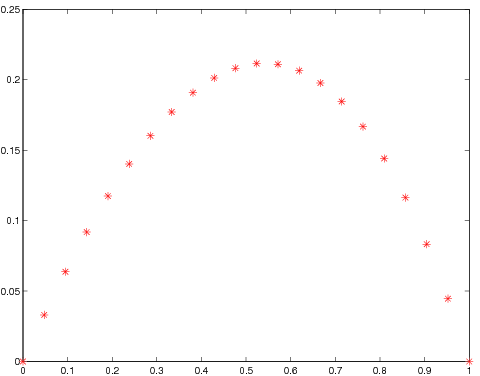
\includegraphics[width=\textwidth]{figures/bild1_27_10}

\column{0.48\textwidth}
\begin{lstlisting}[basicstyle=\tiny]
>> plot(x,z,'r*-','LineWidth',3,'MarkerSize',8)
\end{lstlisting}%
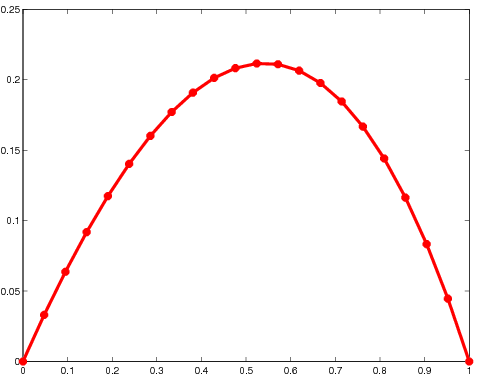
\includegraphics[width=\textwidth]{figures/bild2_27_10}
\end{columns}
\end{frame}

\section{Numerische Lineare Algebra}

\subsection{Normen}
% 
% Slide
%
\begin{frame}[fragile]\frametitle{Vektornorm}
 Die $p$-Norm eines Vektors $x=(x_1, {} \dots , x_n)$
\[ \|x \|_p := \left( \sum_{i=1}^n  |x_i|^p \right)^{1/p} \] 
kann berechnet werden durch \mcode{norm(x,p)} (Default: $p=2$) 
\begin{itemize}
\item Die Norm ist definiert für $p\geq 1$.
\item $p=\infty$ entspricht der Maximum-Norm 
\[  \|x \|_\infty = \max_{i=1, \dots n} |x_i|. \]
\end{itemize}
\end{frame}
% 
% Slide
%
\begin{frame}[fragile]\frametitle{Matrixnorm}
Seien  $A\in \mathbb{C}^{n \times m}$ und
$p \geq 1$. Die
{\it Matrixnorm} ist definiert durch
\[ \| A \|_p = \sup_{x\in \mathbb{C}^m \setminus \{ 0 \}} \frac{\|Ax
  \|_p}{\| x \|_p}. \]
\begin{itemize}
\item In MATLAB:\mcode{norm(A,p)} (Default $p=2$).
\item $p=\infty$ kann charakterisiert werden durch
\[ \|A\|_\infty = \max_{1 \leq j \leq m} \sum_{i=1}^n |a_{ij}|, \quad
\mbox{Zeilensummennorm.} \]
\end{itemize} 
\end{frame}
% 
% Slide
%
\begin{frame}[fragile]\frametitle{Kondition}
Kondition einer quadratischen Matrix $A$: 
{ \[ \cond_p(A):=\|A\|_p\|A^{-1}\|_p. \] }
\vspace*{-0.8cm}
\begin{itemize}
\item In MATLAB: 
  \mcode{cond(A,p)} (Default $p=2$) 
\item Es gilt $\cond_p(A)\geq 1$.
\item Die Kondition mißt die Empfindlichkeit der Lösung $x$ von $Ax=b$
  gegenüber  Störungen
  von $A$ und $b$.
\item Ist $\cond_p(A) >> 1$, so ist die Matrix beinahe singulär. Die Matrix ist {\it schlecht konditioniert}.
\end{itemize}
\end{frame}
% 
% Slide
%
\begin{frame}[fragile]\frametitle{Beispiele}
\begin{itemize}
\item Vektornormen für $x=(1/100) (1, 2, \dots, 100)$
\begin{lstlisting}
>> x = (1:100)/100; [norm(x,1) norm(x,2) norm(x,inf)]
ans =   50.5000    5.8168    1.0000
\end{lstlisting}
\item Matrixnorm für die Hilbert-Matrix $H=(\frac{1}{i+j-1})_{ij}$
\begin{lstlisting}
>> H = hilb(10); [norm(H,1) norm(H,2) norm(H,inf)]
ans =    2.9290    1.7519    2.9290
\end{lstlisting}
\item Kondition der Hilbert-Matrix
\begin{lstlisting}
>> H = hilb(10); [cond(H,1) cond(H,2) cond(H,inf)]
ans =
   1.0e+13 *
    3.5354    1.6025    3.5354
\end{lstlisting}
\end{itemize}
\end{frame}

\subsection{Lösen linearer Gleichungssyteme}
% 
% Slide 
%
\begin{frame}[fragile]\frametitle{Lineare Gleichungssysteme}
Seien $A \in \mathbb{C}^{n\times n}$ und $b \in \mathbb{C}^n$. Das
lineare Gleichungssystem 
{ \[ A x=b \]}
wird in MATLAB gelöst durch  \mcode{ x=A\b}.\\

\begin{lstlisting}
>> x = ones(5,1); H = hilb(5); b = H*x; y = (H\b)'
y =
    1.0000    1.0000    1.0000    1.0000    1.0000
\end{lstlisting}

\alert{Warnung:} Benutze nie
\mcode{x=inv(A)*b}, da das Berechnen von $A^{-1}$ sehr aufwendig sein kann.
\end{frame}
% 
% Slide 
%
\begin{frame}[fragile]\frametitle{LU-Zerlegung}
{\centering  Was bedeutet \mcode{A\b}?}\\[0.5cm]

MATLAB berechnet die LU-Zerlegung von $A$ (Gaussverfahren), d.h.
es sucht eine obere Dreiecksmatrix $U$ und eine untere Dreiecksmatrix
$L$ mit Einsen auf der Diagonalen, so dass $PA=LU$ gilt        
 ($P$ Permutationsmatrix).

Dann wird das LGS durch Rückwärts- und Vorwärtseinsetzen gelöst. 
\begin{lstlisting}
>> [L,U,P]=lu(hilb(5)); norm(P*hilb(5)-L*U)
ans =  2.7756e-17
\end{lstlisting}
\end{frame}
% 
% Slide 
%
\begin{frame}[fragile]\frametitle{Inverse,  Determinante}
\begin{itemize}
\item Berechnung der Inversen
\begin{columns}[onlytextwidth]
\column{0.45\textwidth}
\begin{lstlisting}
>> A=pascal(3)
A =
     1     1     1
     1     2     3
     1     3     6
\end{lstlisting}
\column{0.45\textwidth}
\begin{lstlisting}
>> X=inv(A)
X =
     3    -3     1
    -3     5    -2
     1    -2     1
\end{lstlisting}
\end{columns}
\item Berechnung der Determinante
\begin{lstlisting}
>> det(A)
ans = 1
\end{lstlisting}
\end{itemize}
\end{frame}
% 
% Slide 
%
\begin{frame}[fragile]\frametitle{Pseudoinverse}
Berechnung der (Moore-Penrose) Pseudoinversen $X$ von $A$ ($A$ singulär),
  d.h. $X$ genügt
{ \[ A X A=A,  X A X =X,  (X A)^* =X A,  (A X )^* = A X. \]}
\begin{lstlisting}
>> pinv(ones(3,3))
ans =
    0.1111    0.1111    0.1111
    0.1111    0.1111    0.1111
    0.1111    0.1111    0.1111
\end{lstlisting}
\end{frame}

\subsection{Bestimmung von Eigenwerten}
% 
% Slide 
%
\begin{frame}[fragile]\frametitle{Eigenwerte}
Sei $A \in \mathbb{C}^{n \times n}$. $\lambda \in \mathbb{C}$ ist
Eigenwert von $A$, falls ein Vektor $x \in \mathbb{C}^n$ ungleich $0$ existiert, so
dass  $Ax = \lambda x$ gilt. $x$ heißt Eigenvektor. 
\begin{itemize}
\item {}\mcode{x=eig(A)} berechnet die Eigenwerte von $A$ und schreibt
  sie in den Vektor $x$.
\item
  {}\mcode{[V,D]=eig(A)}
  $D$ ist eine Diagonalmatrix mit den Eigenwerten auf der
  Diagonalen. Die Spalten von $V$ bilden die zugehörigen Eigenvektoren. 
\end{itemize}
\end{frame}
% 
% Slide 
%
\begin{frame}[fragile]\frametitle{Weitere Zerlegungen}
\begin{itemize}
\item Mittels \mcode{[Q,R]=qr(A)} wird zu einer $m \times n$- Matrix
  $A$ eine Zerlegung { $A=QR$} erzeugt,
  wobei $Q$ eine unitäre $m \times m$-Matrix ist und $R$ eine obere
   $m \times n$ Dreiecksmatrix   ist.
\item Eine Singulärwertzerlegung { $A=U \Sigma V^*$} wird durch 
  \mcode{[U,S,V]=svd(A)}
  berechnet. Dabei ist $\Sigma \subset \mathbb{C}^{m \times n}$ eine
  Diagonalmatrix und  $U \subset \mathbb{C}^{m \times m}$, $V \subset
  \mathbb{C}^{n \times n}$  sind unitäre Matrizen. 
\item Eine Cholesky-Zerlegung { $A=R^*R$} 
zu einer hermiteschen, positiv definiten Matrix
  $A$ wird durch  \mcode{R=chol(A)}
  berechnet. $R$ ist eine obere Dreiecksmatrix mit reellen, positiven
  Diagonalelementen. 
\end{itemize}
\end{frame}
% 
% Slide 
%
\begin{frame}[fragile]\frametitle{Bemerkungen}
\begin{itemize}
\item LGS können auch mit Hilfe iterativer Verfahren gelöst werden,
  z.B. \mcode{gmres}, \mcode{pcg}, \mcode{bicgstab}.
\item Ist $A\in \mathbb{C}^{n \times m}$, $n \neq m$, so ergibt \mcode{A\b}
  für $n>m$ (der überbestimmte Fall) die Least-Square Lösung, d.h. der Ausdruck
  \mcode{norm(A*x-b)} wird minimiert. Ist $n<m$ (der unterbestimmte
  Fall) so wird eine Grundlösung berechnet. 
\end{itemize}
\end{frame}
\end{document}